%!TEX root = ../report.tex

% 
% Introduction
% 

\section{Introduction}

Challenges in understanding programs are all too familiar since the early days of computing. At that time we wrote programs in \textit{absolute binary}~\cite{hamming2003art}. It is a numeric representation typically expressed by a sequence of zeros and ones, meaning that the programs were represented as a sequence of instructions and addresses both written in binary. To understand a program in this form is almost impossible.

Since early days, as Fred Brooks pointed out in his influential essay~\cite{bullet1987essence}, we have come to accept that \textit{there is no silver bullet} to understand a program. Fortunately, in recent years, the field of \textit{program comprehension}~\cite{rugaber1995program} has evolved considerably, because, mainly, a program that is not comprehended cannot be changed, shared and communicated.

The area of program comprehension has shown that to understand a program, a \textit{silver bullet} may not be required. This field came up with several theories that provide rich explanations of how people understand programs. For instance, the \textit{top-down} theory~\cite{brooks1977towards} says that to comprehend a program, the programmer must create a mental model of the program's structure and behavior. This model is a set of hypothesis which the programmer confirms or rejects based on evidence found in the code.

In response to these theories or in parallel with them, many environments and innovative tools were created or updated. Some of the examples are: sophisticated frameworks to support rapid construction and integration of tools~\cite{DesRivieres2004}, advanced programming environments with intelligent user interface~\cite{carlson2005eclipse,boudreau2002netbeans,intellij2001intellij,guckenheimer2006software}, and simple tools designed for learning environments~\cite{papert1980mindstorms,Kay1993,Reas2006,findler2002drscheme,GuoSIGCSE2013,mcdirmid2013usable}. In parallel to these advances, there are other fields interested in program comprehension. For example, in the Architecture field, new tools~\cite{aish2012designscript,lopes2011portable} are being proposed to support \textit{generative design}: a procedural method for generating architectural models~\cite{mccormack2004generative}, that also suffers from program understanding problems.

\begin{wrapfigure}{r}{0.4\textwidth}
  \vspace{-20pt}
  \begin{center}
    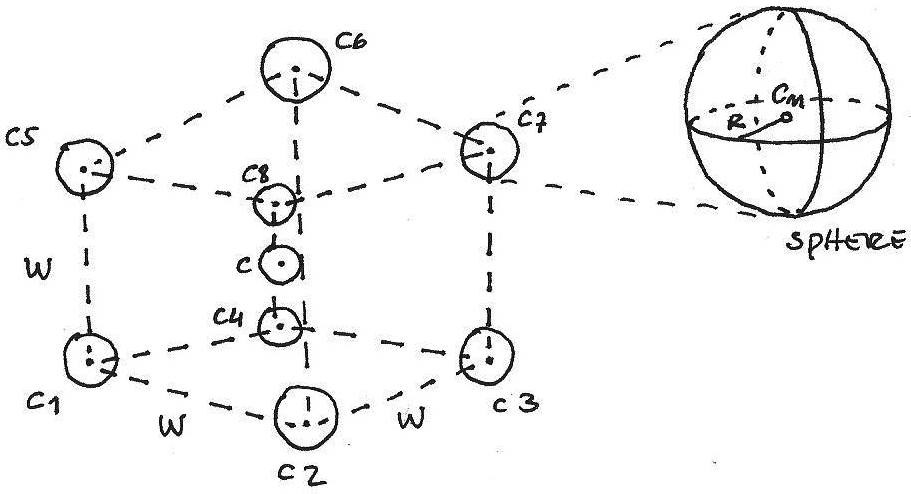
\includegraphics[width=0.4\textwidth]{img/cube-sketch}
  \end{center}
  \vspace{-15pt}
 \caption{An architectural sketch.}  
  \vspace{-20pt}
    \label{fig:sketch}
\end{wrapfigure}

Regardless the area, people follow two steps to build a program: first imagining its details, then implementing them. This is a natural process for programmers that it is commonly performed in their heads. Architects, by contrast, prefer another medium to express their ideas: diagrams/sketches~\cite{do2001thinking}, because it is a compact medium to convey complex ideas. For example, Figure~\ref{fig:sketch} shows a sketch of a geometric model which would be more complex, if it were described in text. These drawings are also helpful in the end of design conception, because they clearly document the design decisions, the relationship between different parts of the design, and the impact of external factors in the final shape.

The generative design programs, by definition, can itself be considered a description of a design, as it formally specifies the modeling process of the design. However, this formal specification can only be easily understood for simple design problems. Consequently, the situation becomes the same of any sufficiently complex program, then it is helpful to have \textit{program documentation}.

In fact many of the discussed problems would be mitigated, if the programs were properly documented. Source code comments is the most important artifact to understand a system and to maintain, as showed in~\cite{de2005study}. Unfortunately, writing documentation is perceived as a tiresome task and, thus, is frequently avoided~\cite{sousa1998survey}, which negatively affects software development. A result of the lack of program documentation is that programmers must spend a significant amount of time separating relevant ideas from the irrelevant ones.

We think that, by creating well designed tools, it is possible to improve \textit{program comprehension} and \textit{program documentation}. We plan to address this problem in two ways: (1) minimizing the lack of documentation in the programs, by turning program documentation in a less tiresome task, and (2) creating a new medium to help people design programs, by anticipating the effect of their actions in the program output.